\section{Architekturen}

\plain{MY-NEUPOWER}

\subsection{MY-NEUPOWER}
\begin{slide}{MY-NEUPOWER}
	\begin{itemize}
		\item von Hitachi Microcomputer System Ltd. (1998)
		\item SIMD parallel Computer
		\item Neuronen als eigene Processing-Elements
		\item Broadcast-Bus zwischen allen PEs
		\item SCSI interface
		\item 25 MHz
		\item 512 physische Neuronen
		\item bis zu 4096 logische Neuronen
	\end{itemize}
\end{slide}

\begin{slide}{MY-NEUPOWER}
	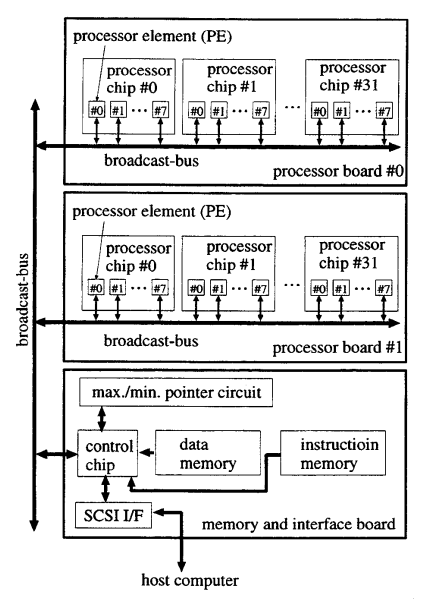
\includegraphics[width=\textwidth,height=0.8\textheight,keepaspectratio]{content/neupower2}
	\blfootnote{Yasunaga, Moritoshi, Akio Yamada, and Tatsuo Okahashi. "Performance of a bus-based parallel computer with integer-representation processors applied to artificial neural network and parallel AI domains." IEEE, 1998.}
\end{slide}

\begin{slide}{MY-NEUPOWER}
	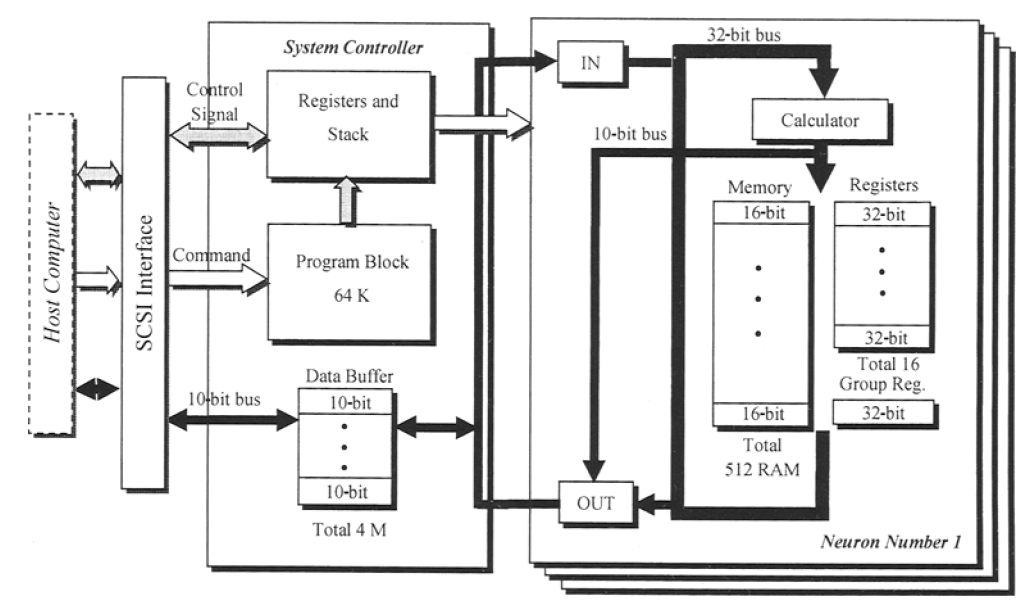
\includegraphics[width=\textwidth,height=0.8\textheight,keepaspectratio]{content/neupower}
	\blfootnote{Sugisaka, Masanori, and Zhi-Jun Liu. "The application of a neurocomputer for a control problem." Artificial Life and Robotics 3.4, 1999.}
\end{slide}

\plain{TrueNorth}
\subsection{TrueNorth}

\begin{slide}{TrueNorth - Idee}
	Die genannten Motive für Neuro-Computer beziehen sich auf aktuelle Forschung und somit auch auf TrueNorth.
	
	Zudem sind die Ziele der TrueNorth Architektur

	\begin{itemize}
		\item Anstelle Modellierung des Gehirns, Nachbildung der Funktionalität
		\item Approximation der Echtzeitverarbeitung des Gehirns
	\end{itemize}
\end{slide}

\begin{slide}{TrueNorth - Architektur}
	Eigenschaften der TrueNorth Architektur ganz im Sinne der genannten Motive.
	
	\begin{itemize}
		\item Skalierbar
		\item Massive Parallelität
		\item Geringer Energieaufwand (slow clock ~1MHz)
		\item Vollständig ereignisgesteuert
		\item Vollständig rekonfigurierbar
	\end{itemize}
\end{slide}

\begin{slide}{TrueNorth - Architektur}
	Die TrueNorth-Architektur baut auf der KNN Terminologie auf. Die CMOS Schaltkreise haben die folgenden Entsprechungen.
	
	\begin{description}
	    \item[Neuronen] Berechnung
	    \item[Synapsen] Speicher (Verbindungsnetzwerk)
	    \item[Axone] Kommunikation (Ausgang)
	    \item[Dendriten] Kommunikation (Eingang)
	\end{description}
\end{slide}

\begin{slide}{TrueNorth - Architektur}
	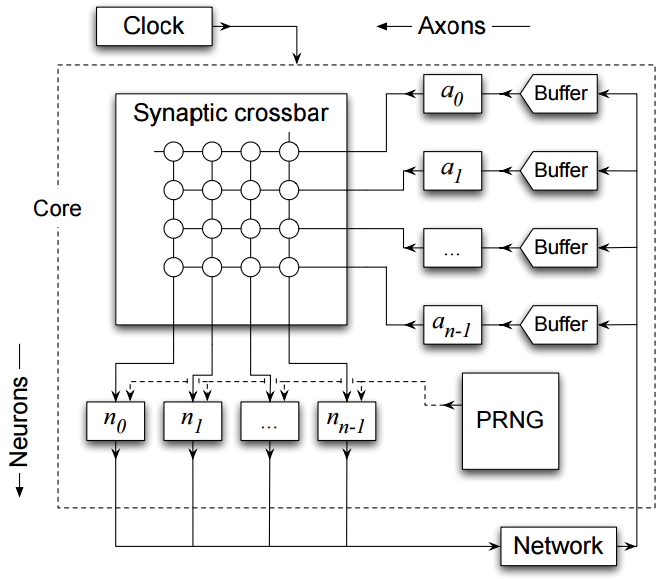
\includegraphics[width=\textwidth,height=0.8\textheight,keepaspectratio]{content/TrueNorthArchitecture.PNG}
\end{slide}

\begin{slide}{Compass}
	Compass ist ein Simulator für die TrueNorth-Architektur.
	
	Simulation auf IBM Blue Gene/Q Supercomputer in Zahlen:
	\begin{itemize}
		\item $262144$ Prozessoren
		\item $256$TB Hauptspeicher
		\item $256 \cdot 10^6$ TrueNorth Kerne
		\item Je Kern $65 \cdot 10^9$ Neuronen
    \item Je Kern $16 \cdot 10^{12}$ Synapsen
	\end{itemize}
\end{slide}

\begin{slide}{Compass}	
	Simulation auf IBM Blue Gene/Q Supercomputer in Zahlen:
	\begin{itemize}
		\item Simuliert damit $3\times$ soviele Neuronen wie geschätzt im Gehirn vorhanden sind
		\item Simulation nur $388\times$ langsamer als Echtzeit
	\end{itemize}
\end{slide}

\plain{Gepulste Neuronale Netze}
\subsection{Gepulste Neuronale Netze}

\begin{slide}{Gepulste Neuronale Netze}
	Gepulste Neuronale Netze sind eine Weiterentwicklung hinsichtlich eines natürlicheren Lernvorgangs.
	
	Hauptmerkmal ist die \alert{Einführung der Zeitabhängigkeit} im Operationszyklus.

	Das bedeutet konkret:
	\begin{itemize}
		\item Schwellenwert zur Aktivierung eines Neurons kann über Zeit erreicht werden
		\item Schwellenwert bleibt erhalten und fällt über Zeit.
	\end{itemize}
\end{slide}

\begin{slide}{Gepulste Neuronale Netze - Architektur}
	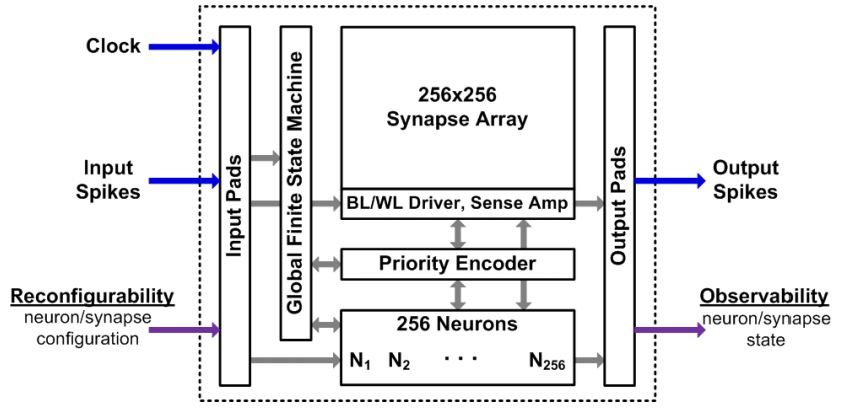
\includegraphics[width=\textwidth,height=0.8\textheight,keepaspectratio]{content/Spiking1.PNG}
\end{slide}

\begin{slide}{Gepulste Neuronale Netze - Neuron}
	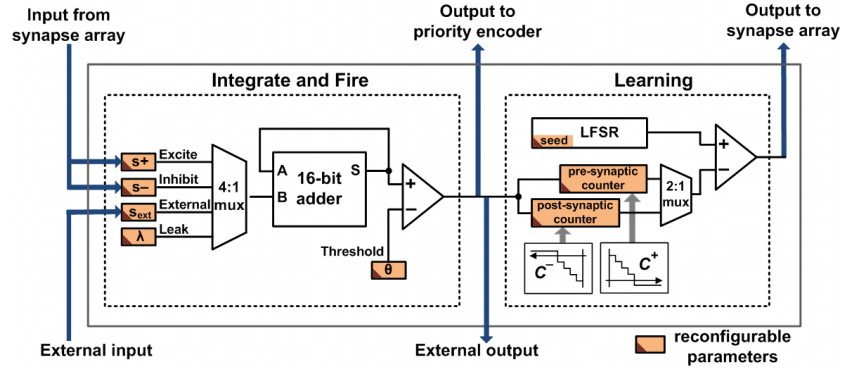
\includegraphics[width=\textwidth,height=0.8\textheight,keepaspectratio]{content/Spiking2.PNG}
\end{slide}
